\newpage
\subsection{Diagrammtypen}

Es gibt verschiedene Diagrammtypen. beispiele dafür sind:

\hfill \break
Das Histogramm:\\
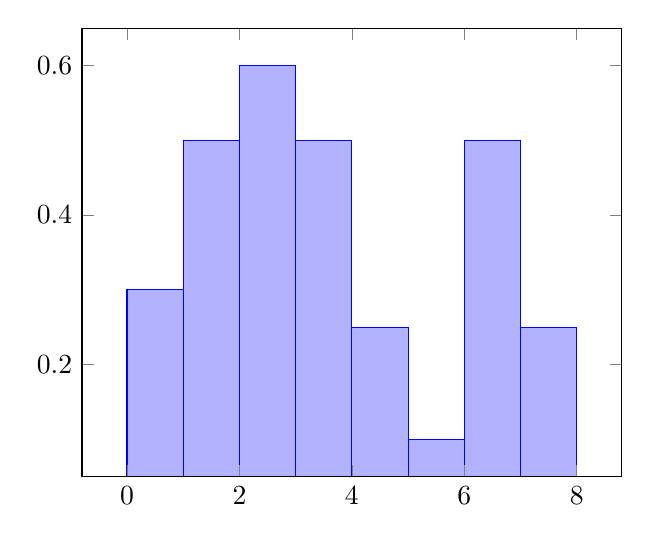
\begin{tikzpicture}
    \begin{axis}[area style]
        \addplot+[ybar interval,mark=no] plot coordinates {
                (0,.3)
                (1,.5)
                (2,.6)
                (3,.5)
                (4,.25)
                (5,.1)
                (6,.5)
                (7,.25)
                (8,.1)
            };
    \end{axis}
\end{tikzpicture}

\hfill \break
Das Kreisdiagramm:\\
\begin{tikzpicture}
    \pie{22.97/Los Angeles Lakers,
        22.97/Boston Celtics,
        8.11/Golden State Warriors,
        8.11/Chicago Bulls,
        6.76/San Antonio Spurs,
        31.07/Other Teams}
\end{tikzpicture}